\section{Introduction}
При построении нейроинтерфейса обычно используются данные сигналов активности головного мозга, представленные в виде многомерных рядов со значениями напряжения на установленных электродах. 

\begin{figure}[h]
	\centering
	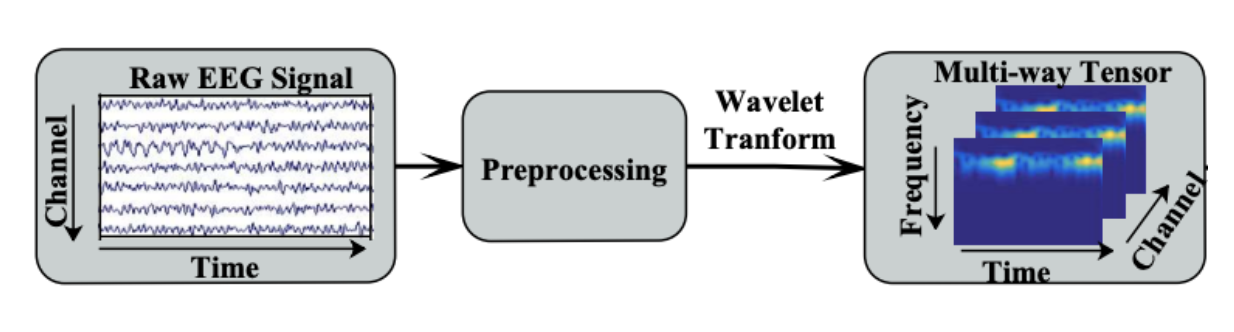
\includegraphics[width=0.9\textwidth]{chapters/varenik2/images/multi-way-eeg.png}
\end{figure}

Такие сигналы естественным образом часто имеют более двух доменов. К времени и пространству добавляется еще частота, получаемая после спектральной предобработки сигнала, помимо этого в одном эксперименте могут учавствовать различные группы испытуемых, использоваться разные условия формирования стимула  и проводиться множество попыток. Использование тензорного представление стало популярным инструментом при работе с биомедицинскими, химическими данными, при обработке сигналов и изображений из-за многомерной структуры таких данных. Поскольку их анализ в матричном виде часто приводит к потере важной информации о существующих связях между представлениями, что приводит к уменьшению полноты признакового описания и, следовательно, ухудшает производительность системы.

\section{References Review}
В книге~\cite{Kolda2009TensorDA} рассматриваются методы тензорного разложения и их применение. В частности, в ней приведены теоретические описания канонически полиадического разложения и расложения Таккера, описаны их свойства и методы вычисления. В статье~\cite{CONG201559} приводится обзор применения тензорного анализа для сигналов EEG, а также описывается обобщение PLS на высокоразмерные тензоры - NPLS с использованием  представления тензора объектов через канонически полиадическое разложение. 
Работа~\cite{6365194} посвящена разработке еще одного обобщения PLS на тензорный случай. В его основе лежит разложение Таккера в композии с канонически полиадическим разложением для обеспечения лучшей аппроксимации исходных данных и единственности разложения при введении условий ортогональности. 

\section{Main Part}
Рассмотрим для начала базовые методы тензорного разложения, такие как каноническое полиадическое разложение и разложение Таккера, которые являются обобщениями матричного SVD для тензорного случая. Они находят широкое применение при анализе многомерных данных в различных приложениях, а именно уменьшение размерности, извлечение и отбор признаков для построения устойчивой модели, анализ независимых компонент и полезны в интерпретации для обеспечения связей между извлеченными факторами и их физиологическими значениями.

\subsection{Канонически полиадическое разложение (CP decomposition)}

\textbf{3-way}

Рассмотрим для начала трехмерный случай, а потом обобщим на N-мерный.
Пусть $\vect X \in \mathbb{R}^{I\times J \times K}$ - тензор 3-го порядка. Каноническое полиадическое разложение $\vect X$ есть линейная комбинация тензоров единичного ранга (внешних произведений векторов):
\begin{gather}
    \vect X \approx [\bm{\lambda}; \vect A, \vect B, \vect C] \equiv \sum\limits_{r=1}^R \lambda_r \vect a_r \circ \vect b_r \circ \vect c_r, \text{ } \vect a_r \in \mathbb{R}^I, \vect b_r \in \mathbb{R}^J, \vect c_r \in \mathbb{R}^K, \lambda_r \in \mathbb{R},
    \label{eq1}
\end{gather}
$\vect A \in \mathbb{R}^{I\times R}, \vect B \in \mathbb{R}^{J\times R}, \vect C \in \mathbb{R}^{K\times R} - \text{фактор-матрицы}$.
	
\begin{figure}[h]
	\centering
	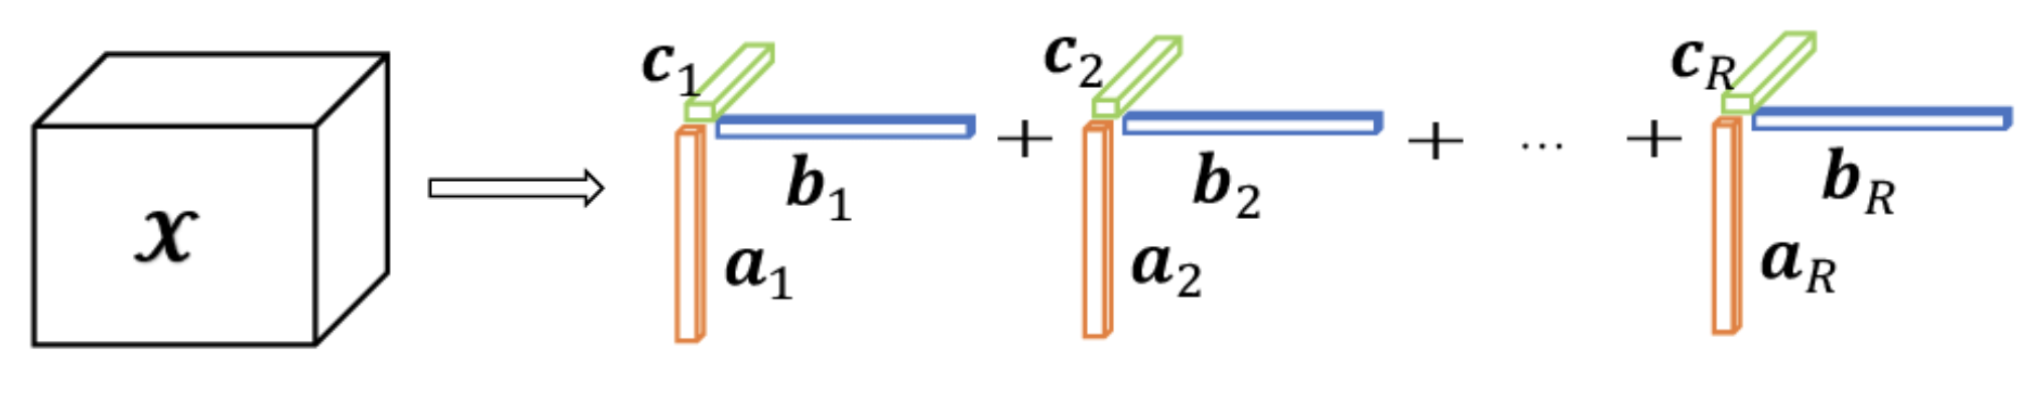
\includegraphics[width=0.95\textwidth]{chapters/varenik2/images/cp-decomposition.png}
\end{figure}
    
Для канонически полиадического разложения задается осевая матризация, для трехмерного случая она имеет вид:
\begin{gather*}
    \vect X_{(1)} \approx \vect A diag(\bm{\lambda})(\vect C\odot \vect B)^T,\\
    \vect X_{(2)} \approx \vect B diag(\bm{\lambda})(\vect C\odot \vect A)^T,\\
    \vect X_{(3)} \approx \vect C diag(\bm{\lambda})(\vect B\odot \vect A)^T.
\end{gather*}
    
Матризация тензора это механизм раскладки тензора в матрицу. Есть осевая матризация, в которой рассматриваются трубки тензора, задаваемые элементами со всеми зафиксированными осями кроме одной - рассматриваемой. Тогда $n$-я осевая матризованная форма $\vect X_{(n)}$ тензора $\vect X \in \mathbb{R}^{I_1\times I_2 \times \dots \times I_N}$ определяется как матрица, в которой столбцы задаются трубками $\vect x_{i_1\dots i_{n-1}\textbf{:}i_{n+1}\dots i_N}$. Еще один тип матризации - на основе срезов (или слайсов), в которой тензор делится на панельки, определяемые элементами со всеми зафиксированными осями, кроме двух. Аналогично осевой матризации, выделенные срезы выстраиваются в матрицу в виде блочных столбцов. В дальнейшем ограничимся только осевой матризацией.

\begin{figure}[h]
	\centering
	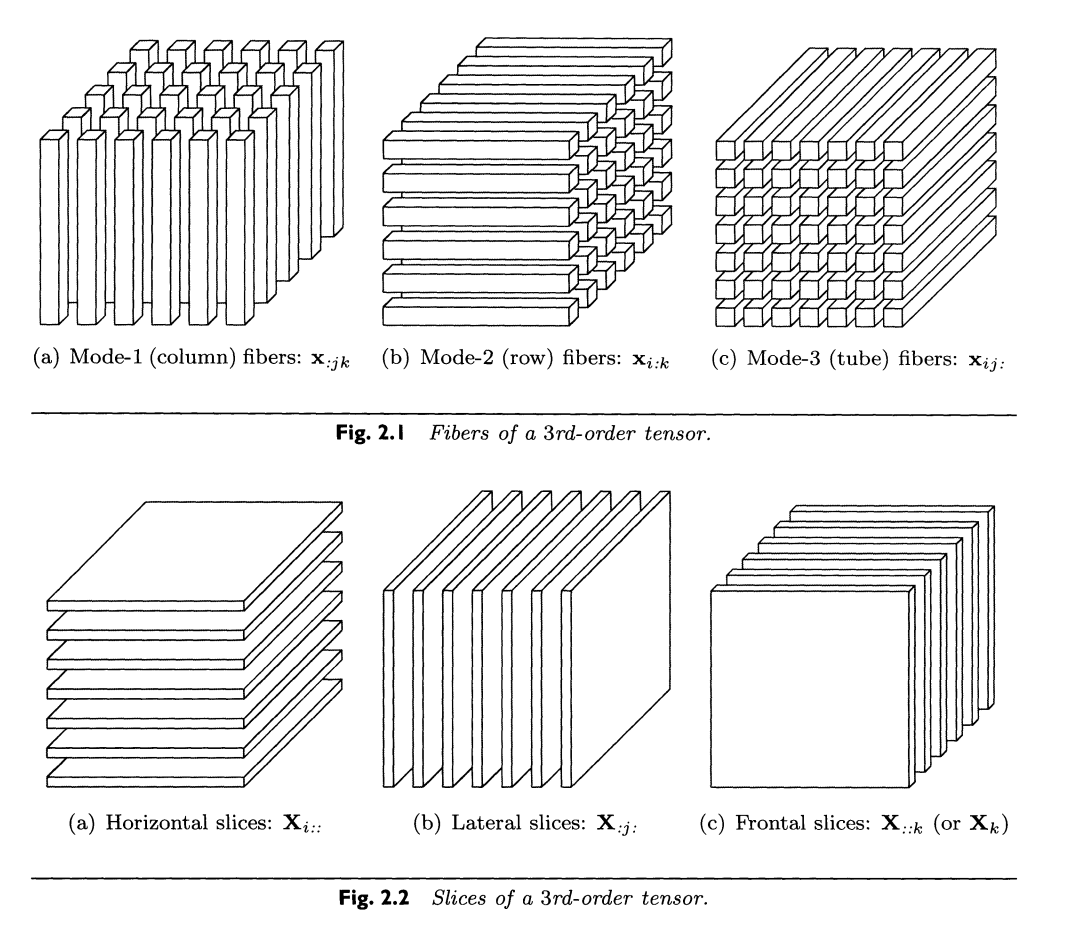
\includegraphics[width=0.7\textwidth]{chapters/varenik2/images/matricization.png}
\end{figure}

\textbf{Свойства}

\begin{itemize}
    \item $rank \vect X$ - наименьшее R необходимое для точной аппроксимации в (\ref{eq1}) при заданном уровне точности разложения;
    \item единственность разложения - при инвариантности к:
        \begin{align*}
            & 1)\text{перестановкам } \vect X = [\bm{\lambda}; \vect A, \vect B, \vect C] = [\bm{\lambda}; \vect A\vect P, \vect B\vect P, \vect C\vect P], \text{ }\vect P \in \mathbb{R}^{R\times R},\\
            & 2)\text{масштабированию } \vect X = \sum_{r=1}^R \lambda_r (\alpha_r \vect a_r) \circ (\beta_r \vect b_r) \circ (\gamma_r \vect c_r), \text{ } \alpha_r\beta_r\gamma_r = 1;
        \end{align*}
    \item вычисляется альтернативным методов наименьших квадратов:
    \begin{align*}
        \min_{\hat{\vect X}} ||\vect X - \hat{\vect X}||_F, \text{где }
        \hat{\vect X} = \sum\limits_{r=1}^R \lambda_r \vect a_r \circ \vect b_r \circ \vect c_r;
    \end{align*}
\end{itemize}

Идея в том, чтобы зафиксировать все фактор-матрицы кроме одной и рассматривать задачу минимизации ошибки аппроксимации относительно незафиксированной матрицы, а затем то же самое повторить для остальных фактор-матриц. Ниже приведет алгоритм вычисления подходящих фактор-матриц и вектора коэффициентов. Он состоит из инициализации и повторения шагов пересчета до тех пор, пока не будет выполнен остановочный критерий. Вектор коэффициентов получается из нормировки фактор-матриц ввиду условия, что их компоненты должны иметь единичную норму.

\begin{figure}[h]
	\centering
	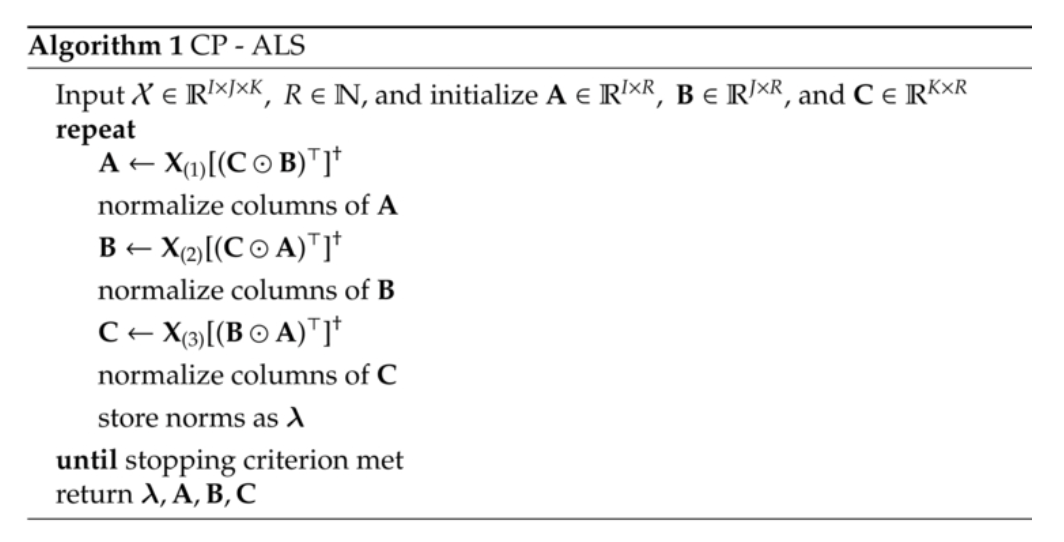
\includegraphics[width=0.8\textwidth]{chapters/varenik2/images/cp-als.png}
\end{figure}

\textbf{N-way}

Пусть $\vect X \in \mathbb{R}^{I_1\times I_2 \times \dots \times I_N}$ - тензор N-го порядка. Тогда канонически полиадическое разложение определяется как:
\begin{gather}
    \vect X \approx \sum\limits_{r=1}^R \lambda_r \vect a_r^{(1)} \circ \vect a_r^{(2)} \circ \dots \circ \vect a_r^{(N)} = [\bm{\lambda}; \vect A^{(1)}, \vect A^{(2)}, \dots, \vect A^{(N)}],
\end{gather}
$$\vect a_r^{(n)} \in \mathbb{R}^{I_n}, ||\vect a_r^{(n)}||_2 = 1, \forall n \in \overline{1, N}.$$
        
При этом осевая матризация:
\begin{gather*}
    \vect X_{(n)} \approx \bm{\Lambda} (\vect A^{(N)} \odot \dots \odot \vect A^{(n+1)} \odot \vect A^{(n-1)} \odot \dots \odot \vect A^{(1)})\vect A^{(n)T}, \text{ } \bm{\Lambda} = diag(\bm{\lambda}).
\end{gather*}

\subsection{Разложение Таккера (Tucker decomposition)}
\textbf{3-way}

Пусть $\vect X \in \mathbb{R}^{I\times J \times K}$ - тензор 3-го порядка. Разложение Таккера предствляет $\vect X$ в виде набора ядра и трех ортогональных фактор-матриц. Такое представление позволяет извлекать информацию о взаимосвязи между различными осевыми компонентами в разложении:
\begin{gather}
    \vect X \approx \vect G \times_1 \vect A \times_2 \vect B \times_3 \vect C = \sum\limits_{r_a=1}^{R_A}\sum\limits_{r_b=1}^{R_B}\sum\limits_{r_c=1}^{R_C} g_{r_a r_b r_c} \vect a_{r_a} \circ \vect b_{r_b} \circ \vect c_{r_c} = [\vect G; \vect A, \vect B, \vect C],
    \label{eq2}
\end{gather}
$\vect A \in \mathbb{R}^{I\times R_A}, \vect B \in \mathbb{R}^{J\times R_B}, \vect C \in \mathbb{R}^{K\times R_C} - \text{фактор-матрицы}$, которые могут рассматриваться как главные компоненты каждой оси, 
$\vect G\in \mathbb{R}^{R_A\times R_B \times R_C}$ - ядро, отображающее уровень взаимодействия между разными компонентами.

\begin{figure}
	\centering
	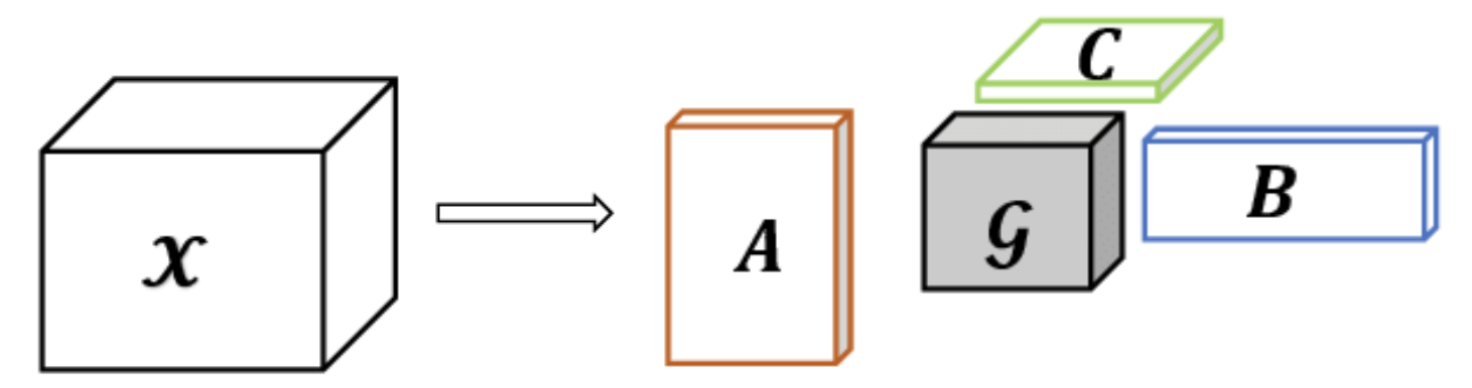
\includegraphics[width=0.72\textwidth]{chapters/varenik2/images/tucker-decomposition.png}
\end{figure}

Матризованная форма:
\begin{gather*}
    \vect X_{(1)} \approx \vect A \vect G_{(1)}(\vect C\otimes \vect B)^T,\\
    \vect X_{(2)} \approx \vect B \vect G_{(2)}(\vect C\otimes \vect A)^T,\\
    \vect X_{(3)} \approx \vect C \vect G_{(3)}(\vect B\otimes \vect A)^T.
\end{gather*}
  
\textbf{Свойства}

\begin{itemize}
    \item частичный ранг $rank_n \vect X$ - количество столбцов матрицы $\vect X_{(n)}$;
    \item при $\vect B = \vect I, \vect C = \vect I$ соответствует стандартному двумерному PCA: $\vect X_{(1)} = \vect A \vect G_{(1)}$;
    \item вычисляется методом HOSVD:
    \begin{align*}
        \min_{\vect G, \vect A, \vect B, \vect C} ||\vect X - [\vect G; \vect A, \vect B, \vect C]_{\text{Tucker}}||_F;
    \end{align*}
\end{itemize}

\begin{figure}[h]
	\centering
	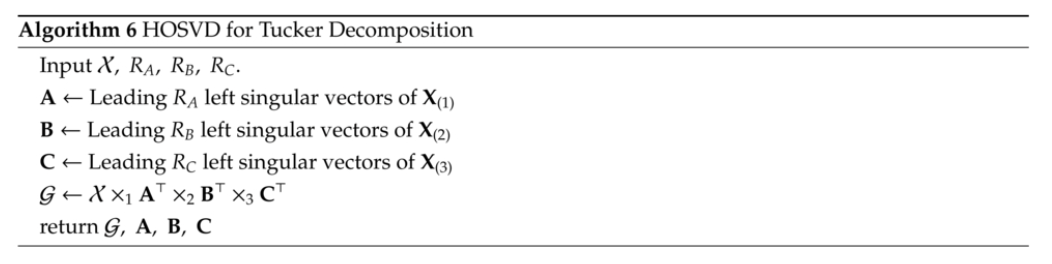
\includegraphics[width=0.95\textwidth]{chapters/varenik2/images/hosvd.png}
\end{figure}
    
\textbf{N-way}

Аналогично определяется $N$-мерное расширение разложения Таккера, которое представляет собой матричное произведение ядра на $N$ фактор матрицы.

Пусть $\vect X \in \mathbb{R}^{I_1\times I_2 \times \dots \times I_N}$, тогда:
\begin{gather*}
    \vect X = \vect G \times_1 \vect A^{(1)} \times_2 \vect A^{(2)} \times_3 \dots \times_N \vect A^{(N)} = [\vect G; \vect A^{(1)}, \vect A^{(2)}, \dots, \vect A^{(N)}],\\
    \vect X_{(n)} = \vect A^{(n)} \vect G_{(n)} (\vect A^{(N)} \otimes \dots \otimes \vect A^{(n+1)} \otimes \vect A^{(n-1)}\otimes \dots \otimes \vect A^{(1)})^T.
\end{gather*}


Таким образом, CP обладает свойством уникальности при достаточно слабых условиях, но при этом пренебрегает взаимодействием между компонентами в разных осях.
Разложение Таккера в общем случае неединственно, что затрудняет интерпретацию полученной скрытой структуры данных, но при этом является обобщением CP разложения для возможности учета информации о взаимных связях.
    
\subsection{Обобщение PLS на тензорный случай: N-way PLS и HOPLS}

\textbf{Standard PLS}

В системах BCI, в задачах регрессии линейные модели применяются в основном из-за их простоты и надежности, при этом высокая размерность данных затрудняет прямое применение общих методов линейной регрессии. Регрессия методом частичных наименьших квадратов как раз подходит для таких ситуаций.

Решая задачу методом частничных наименьших квадратов проблема сводится к нахождению общего скрытого пространства, одновременно хорошо аппроксимирующего $X$ и $Y$.

Метод PLS раскладывает исходную матрицу на произведение матрицы представления в скрытом пространстве и матрицы перехода, что можно также записать в виде суммы матриц единичного ранга.

\begin{gather*}
    \vect X = \vect T \vect P^T + \vect E = \sum_{r=1}^R \vect t_r \vect p_r^T + \vect E, \text{ }\vect X \in \mathbb{R}^{I\times J} - \text{матрица объектов}\\
    \vect Y = \vect U \vect Q^T + \vect F = \sum_{r=1}^R \vect u_r \vect q_r^T + \vect F, \text{ }\vect Y \in \mathbb{R}^{I\times M} - \text{матрица ответов},
\end{gather*}
$\vect T, \vect U \in \mathbb{R}^{I\times R}$ - матрицы описания $\vect X$ и $\vect Y$ в скрытом пространстве,\\ 
$\vect P \in \mathbb{R}^{J\times R}, \vect Q \in \mathbb{R}^{M\times R}$ - матрицы перехода в скрытое пространство, \\
$\vect E \in \mathbb{R}^{I\times J}, \vect F \in \mathbb{R}^{I\times M}$ - матрицы невязок.

В предположении наличия линейной связи $\vect u \approx d\vect t$, получаем задачу нахождения совместной матрицы Т, наилучшим образом описывающей исходные $X$ и $Y$:
\begin{gather*}
    \vect Y = \vect T \vect D \vect Q^T + \vect F = \sum_{r=1}^R d_{rr}\vect t_r \vect q_r^T + \vect F, \text{ } \vect D = diag(d_{rr}), \text{ } d_{rr} = \frac{\vect u_r^T \vect t_r}{\vect t_r^T \vect t_r}
\end{gather*}

\begin{figure}[h]
	\centering
	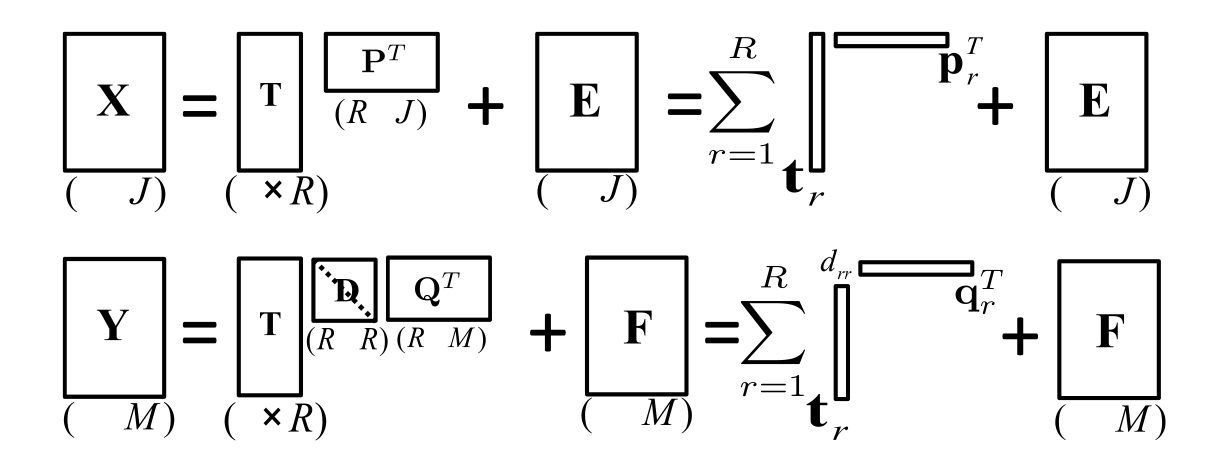
\includegraphics[width=0.7\textwidth]{chapters/varenik2/images/pls.png}
\end{figure}

\newpage
\textbf{N-way PLS}

Для тензорного случая имеется простое прямое обобщение PLS. А именно, пусть имеется тензор объектов 4 порядка $\vect X \in \mathbb{R}^{I\times L\times K\times J}$, и матрица ответов $\vect Y \in \mathbb{R}^{I\times N}$. Тогда с использованием CP разложения NPLS принимает вид, в котором $X$ представляется в виде суммы внешних произведений скрытого вектора на векторы перехода, соответствующие отдельным признаковым доменам. Поскольку Y -  матрица, ее разложение определяется стандартным образом:
\begin{gather*}
    \vect X = \sum\limits_{r=1}^R \vect t_r \circ \vect p_r \circ \vect q_r \circ \vect s_r + \vect E,\\
    \vect Y = \sum\limits_{r=1}^R d_{rr}\vect t_r \vect c_r^T + \vect F, \text{где}
\end{gather*}
$\vect t_r \in \mathbb{R}^{I\times 1}$ - скрытый вектор, $\vect p_r \in \mathbb{R}^{L\times 1}, \vect q_r \in \mathbb{R}^{K\times 1}, \vect s_r \in \mathbb{R}^{J\times 1}$ - векторы перехода.\\~\

При NPLS оговаривается, что $\forall r = 1, \dots R$ векторы $\vect p, \vect q, \vect s, \vect c$ определяются из условия максимизации ковариации между скрытыми представлениями:
\begin{gather*}
    [\vect p, \vect q, \vect s, \vect c] = \arg \max_{\vect p, \vect q, \vect s, \vect c} [cov(\vect t, \vect u)], \text{ при}\\
    t_i = \sum\limits_{l=1}^L\sum\limits_{k=1}^K\sum\limits_{j=1}^J x_{ilkj}p_l q_k s_j = \vect y_i \vect c, \text { и }
    ||\vect p||_2^2 = ||\vect q||_2^2 = ||\vect s||_2^2 = 1
\end{gather*}

\textbf{HOPLS}

Рассмотрим еще одно обобщение PLS, называемое HOPLS. В нем используется разложение Таккера для отображения более сложных зависимостей. Его использование обосновывается фактом, что разложение Таккера является ранговой подпространственной аппроксимацией в отличии от CP, которое является простой аппроксимацией низшего ранга. Исходя из этого в работе предполагается, что модель на основе разложения Таккера лучше справляется с аппроксимацией данных.

\begin{figure}
	\centering
	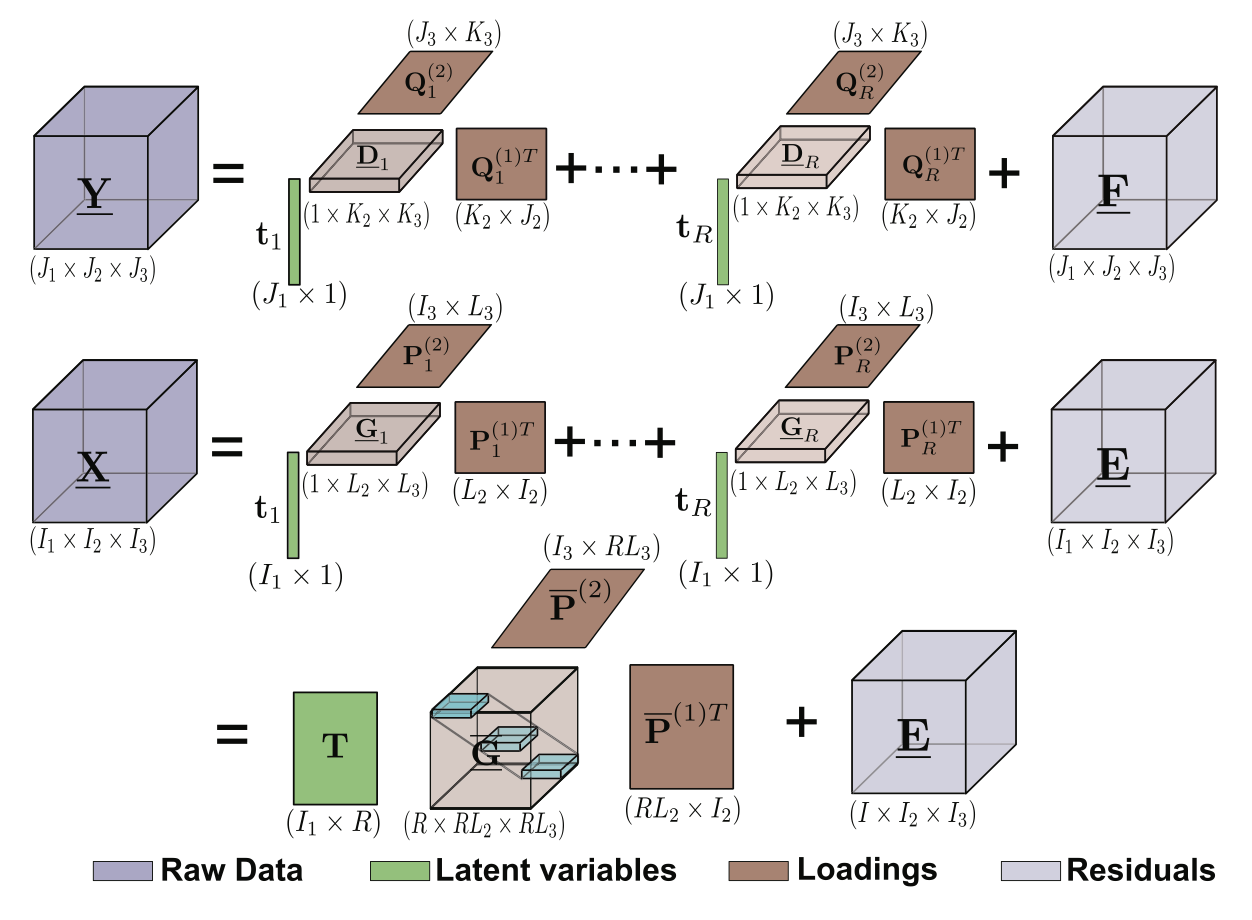
\includegraphics[scale=0.55]{chapters/varenik2/images/hopls.png}
\end{figure}
 
Заметим, что используется не стандартное разложение Таккера, а его комбинации с CP разложением. В итоге, исходный тензор представляется в виде суммы блоков Таккера, которые потом объединяются в общее представление с блочнодиагоальным ядром.

Пусть $\vect X \in \mathbb{R}^{I_1\times \dots \times I_N}, \vect Y \in \mathbb{R}^{J_1\times \dots \times J_M}$, при этом $I_1 = J_1$. Модель HOPLS определяется как: 
\begin{gather*}
    \vect X = \vect G \times_1 \vect T \times_2 \vect P^{(1)} \times_3 \dots \times_N \vect P^{(N-1)} + \vect E,\\
    \vect Y = \vect D \times_1 \vect T \times_2 \vect Q^{(1)} \times_3 \dots \times_M \vect Q^{(M-1)} + \vect F, 
\end{gather*}
где ядро-тензоры
\begin{gather*}
    \vect G = blockdiag(\vect G_1, \dots, \vect G_R) \in \mathbb{R}^{R\times RL_2 \times \dots \times RL_N},\\
    \vect D = blockdiag(\vect D_1, \dots, \vect D_R) \in \mathbb{R}^{R\times RK_2 \times \dots \times RK_M},
\end{gather*}
$\vect T\in \mathbb{R}^{I_1\times R}$ - матрица скрытых переменных,\\
$\vect P^{(n)} = [\vect P_1^{(n)}, \dots, \vect P_R^{(n)}]$, $\vect Q^{(m)} = [\vect Q_1^{(m)}, \dots, \vect Q_R^{(m)}]$ - матрицы перехода для оси $n$ и $m$ соответственно.

\textbf{Применение}

Что касается применения к декодированию, в работе HOPLS проводилось исследование по сравнению стандартного PLS, NPLS и HOPLS в задаче прогнозирования движения руки в 3-мерном пространстве по 4 маркерам установленным на руке, запястье, локте и плече. В качестве данных использовались электрокортикограммы, которые рассматривались в 4 доменах: эпоха, время, частота, пространство. Были получены результаты в которых HOPLS значимо превосходит своих предшественников, при этом исходя из посчитанной точности видно, что NPLS не гарантирует лучшей производительности по сравнению со стандартным матричным подходом.

\begin{figure}[h]
    \centering
    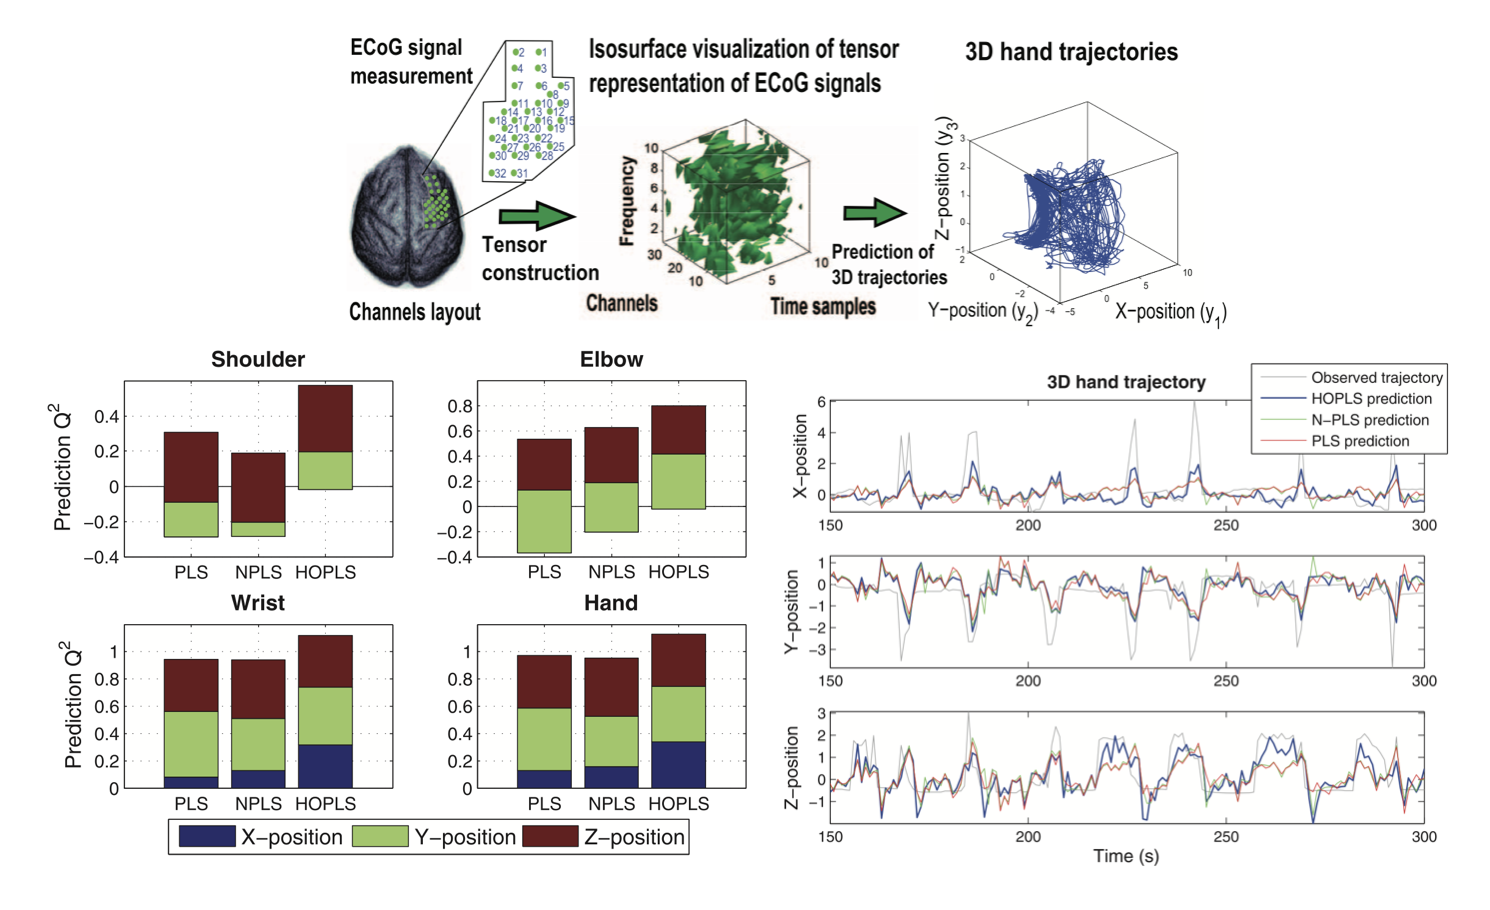
\includegraphics[scale=0.65]{chapters/varenik2/images/result.png}
\end{figure}

\section{Questions To Discussion}
\begin{enumerate}
    \item Чем отличаются конструкции CP и Tucker разложения?
    \item При каком условии одно разложения является частным другого?
    \item Какой общий принцип используется для вычисления разложений?
    \item В чем состоит подход альтернативного метода наименьших квадратов для CP разложения?
    \item Чем объясняется очевидность обобщения стандартного PLS до NPLS?
\end{enumerate}